\documentclass[xcolor=table, 10pt, aspectratio=169]{beamer}
% !TEX engine = xelatex
%\usepackage{times}
%\usefonttheme{serif}
\usepackage{amsmath,amssymb,amscd}
\usepackage{dsfont}
\usepackage{mathrsfs}
\usepackage{yfonts}
\usepackage{bm}
\usepackage{graphicx}
\usepackage{tabularx}
\usepackage{animate}
\usepackage{pifont}
%\usepackage{ifthen}

\usepackage{xeCJK}
\usepackage{fontspec}
%\newfontfamily\cjkfont{PingFang SC}
\setCJKmainfont{PingFang SC}
%\newfontfamily\cjkfont{Songti SC}
%\newfontfamily\cjkfont{STSong}
%\setCJKmainfont{Songti SC}
%\setCJKmainfont{STSong}
\newcolumntype{x}{>{\centering\arraybackslash}X}
\renewcommand{\arraystretch}{1.5}

\usepackage{tikz}
	\usetikzlibrary{calc}
	\usetikzlibrary{arrows,shapes, positioning, matrix}
	\usetikzlibrary{decorations.markings}
	\tikzstyle arrowstyle=[scale=1]
	\tikzstyle directed=[postaction={decorate,decoration={markings,
 	   mark=at position .15 with {\arrow[arrowstyle]{stealth}}}}]
\tikzstyle string=[thick,postaction={decorate,decoration={markings,
    mark=at position .55 with {\arrow[arrowstyle]{stealth}}}}]
\tikzstyle dual_string=[dashed,postaction={decorate,decoration={markings,
    mark=at position .55 with {\arrow[arrowstyle]{stealth}}}}]

\tikzstyle dw=[thick,postaction={decorate,decoration={markings,
    mark=at position 1 with {\arrow[arrowstyle]{stealth}}}}]
\tikzstyle group=[mbg]

\usepackage{pgffor}
\newcommand{\mb}[1]{\mathbf{#1}}
\renewcommand{\cal}[1]{\mathcal{#1}}

\newcommand{\ag}[2]{#1_\mb{#2}}
\newcommand{\cohosub}[1]{\scalebox{0.72}{\textswab{#1}}}
\newcommand{\cohosubsub}[1]{\scalebox{0.6}{\textswab{#1}}}
\newcommand{\coho}[1]{\textswab{#1}}


\mode<presentation>
{
  %\usetheme{Warsaw}
  % or ...
  %\useoutertheme{rectangle}
  \setbeamertemplate{frametitle}[default][center]
  \defbeamertemplate{itemize item}{flat}{\begin{pgfpicture}{-1ex}{0ex}{1ex}{2ex}
      \pgfpathcircle{\pgfpoint{0pt}{.6ex}}{0.6ex}
      \pgfusepath{fill}
    \end{pgfpicture}%
  }
  \defbeamertemplate{itemize subitem}{flat}{\footnotesize\raise0.5pt\hbox{\textbullet}}
  \defbeamertemplate{itemize subsubitem}{flat}{\footnotesize\raise0.5pt\hbox{\textbullet}}

  %\useinnertheme{circles}
  \setbeamertemplate{items}[flat]
  \setbeamertemplate{sections/subsections in toc}[circle]
  \setbeamertemplate{blocks}[rounded]
  \setbeamertemplate{title page}[default][colsep=-4bp,rounded=true]
  \setbeamertemplate{part page}[default][colsep=-4bp,rounded=true]
  \setbeamercovered{transparent}
  %\usecolortheme{spruce}
  %\definecolor{THU}{RGB}{116,61,130}
  \definecolor{mbg}{RGB}{0,0,160}
  \setbeamercolor*{palette primary}{fg=white,bg=mbg}
  \setbeamercolor*{titlelike}{parent=palette primary}
  \setbeamercolor*{structure}{fg=mbg}
  \setbeamercolor{frametitle}{fg=white,bg=mbg}
  % or whatever (possibly just delete it)
  \setbeamercolor{block title}{bg=mbg,fg=white}
  \setbeamercolor{block body}{bg=mbg!15}


  \addtobeamertemplate{navigation symbols}{}{ \hspace{1em}%
    \usebeamerfont{footline}%
    \insertframenumber / \inserttotalframenumber }
}


%\usepackage[english]{babel}
% or whatever

%\usepackage[latin1]{inputenc}
% or whatever

%\usepackage{times}
%\usepackage[T1]{fontenc}
% Or whatever. Note that the encoding and the font should match. If T1
% does not look nice, try deleting the line with the fontenc.

\title[EQMC] % (optional, use only with long paper titles)
{Metal to Orthogonal Metal Transition}

\author[Y Qi] % (optional, use only with lots of authors)
{Yang~Qi}
% - Give the names in the same order as the appear in the paper.
% - Use the \inst{?} command only if the authors have different
%   affiliation.

\institute[Fudan] % (optional, but mostly needed)
{
Department of Physics, Fudan University.
}
% - Use the \inst command only if there are several affiliations.
% - Keep it simple, no one is interested in your street address.

%\date{2016 Annual Meeting of Fudan CFTPP} % (optional, should be abbreviation of conference name)
%{Fudan University, Oct 13 2015}
\date{SUSTech, May 17th 2019.}
% - Either use conference name or its abbreviation.
% - Not really informative to the audience, more for people (including
%   yourself) who are reading the slides online

\subject{Theoretical Physics}
% This is only inserted into the PDF information catalog. Can be left
% out.



% If you have a file called "university-logo-filename.xxx", where xxx
% is a graphic format that can be processed by latex or pdflatex,
% resp., then you can add a logo as follows:

\pgfdeclareimage[height=1cm]{university-logo}{../resources/fudan}
\logo{\pgfuseimage{university-logo}}

\begin{document}

%\begin{frame}
%  \titlepage
%\end{frame}

\begin{frame}{Metal to Orthogonal Metal Transition}
\begin{itemize}
\item 陈闯, 中科院物理所.
\item 许霄琰, 香港科技大学$\rightarrow$University of California at San Diego.
\item 孟子杨, 中科院物理所/香港大学.
\begin{center}
  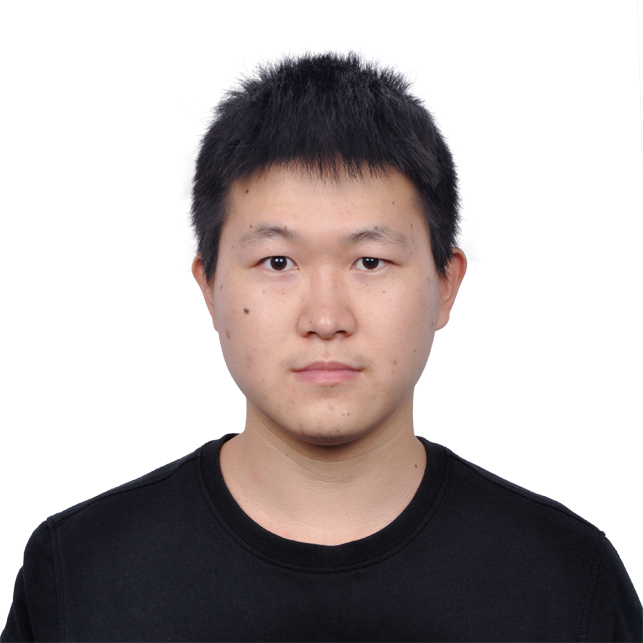
\includegraphics[height=2.5cm]{../people/chuangchen}
  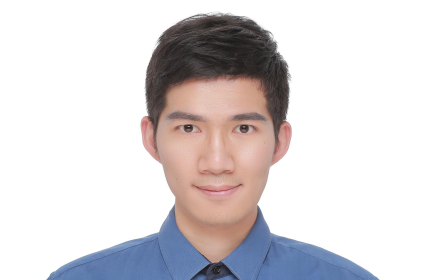
\includegraphics[height=2.5cm]{../people/xiaoyanxu}
  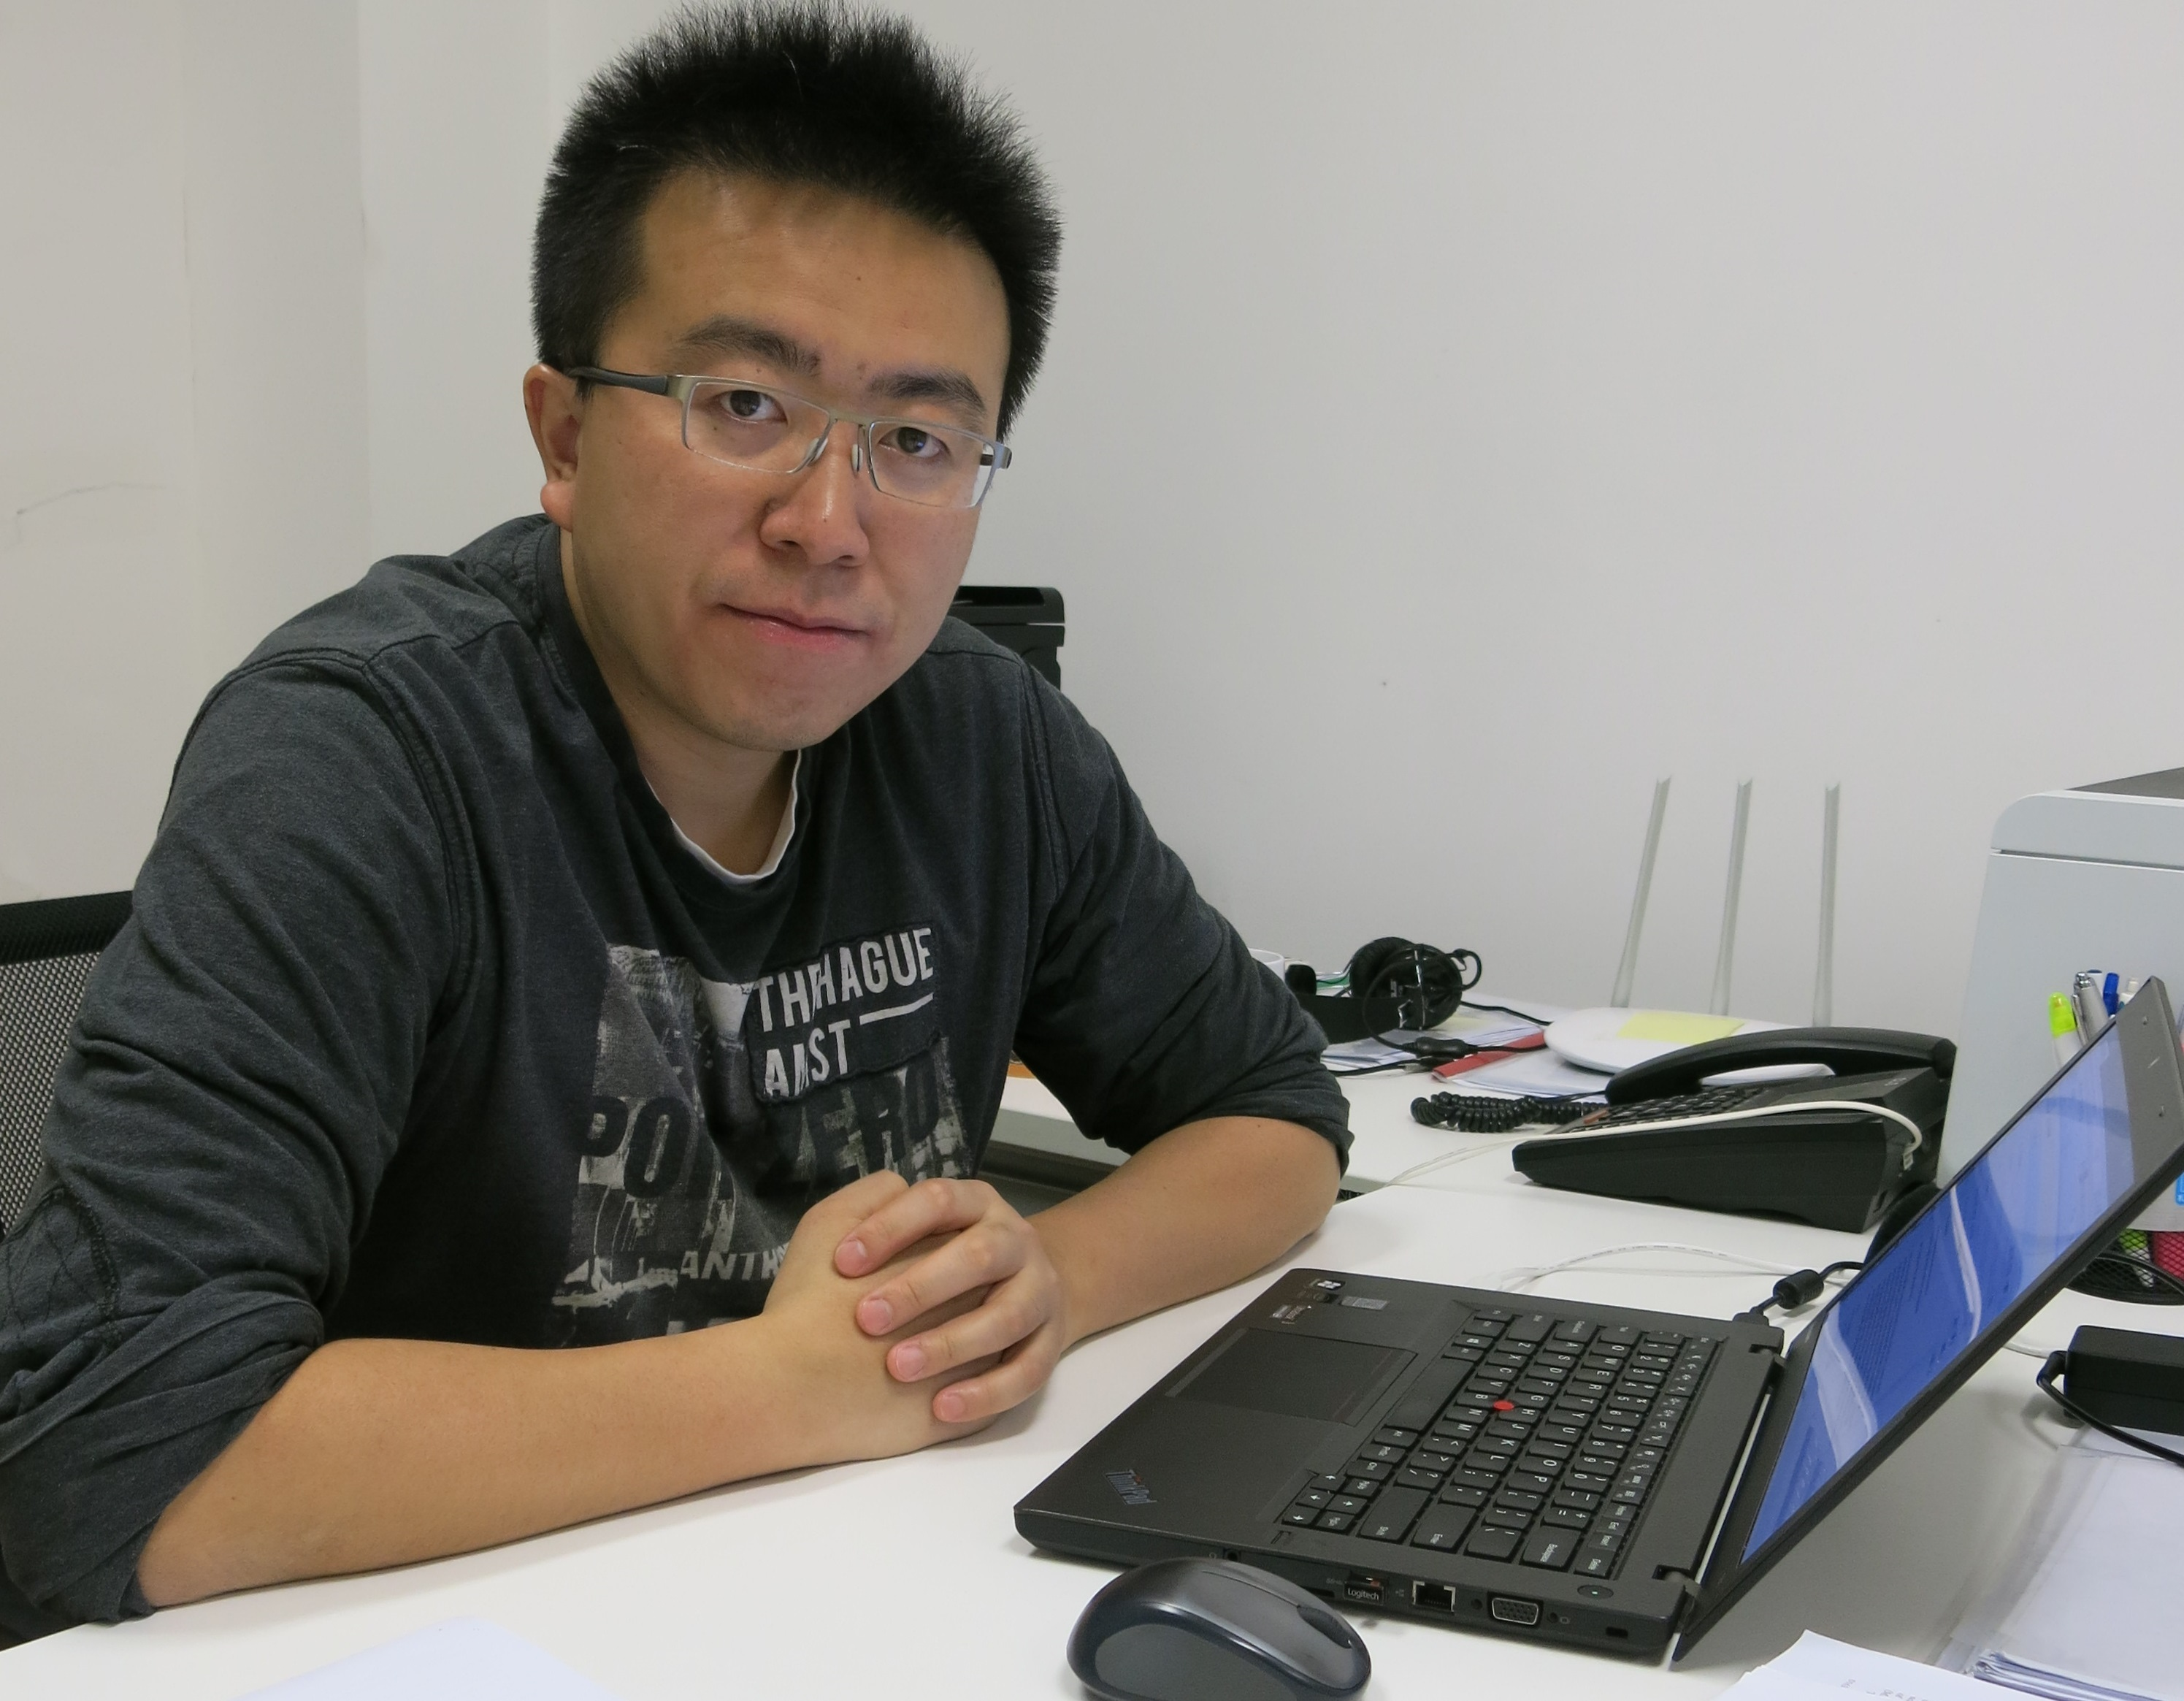
\includegraphics[height=2.5cm]{../people/ziyangmeng}
\end{center}
\end{itemize}
\begin{center}
  中国物理快报, \textbf{37}(4), 047103 (2020).
\end{center}
\end{frame}

\section{Introduction}

\begin{frame}
  \frametitle{正常金属:费米面}
\begin{itemize}
  \item 根据朗道费米液体理论,即使考虑了相互作用的效果,金属中也存在费米面。
  \item Luttinger定理保证即使在相互作用修正下,费米面的大小仍保持不变。
\end{itemize}
\begin{center}
	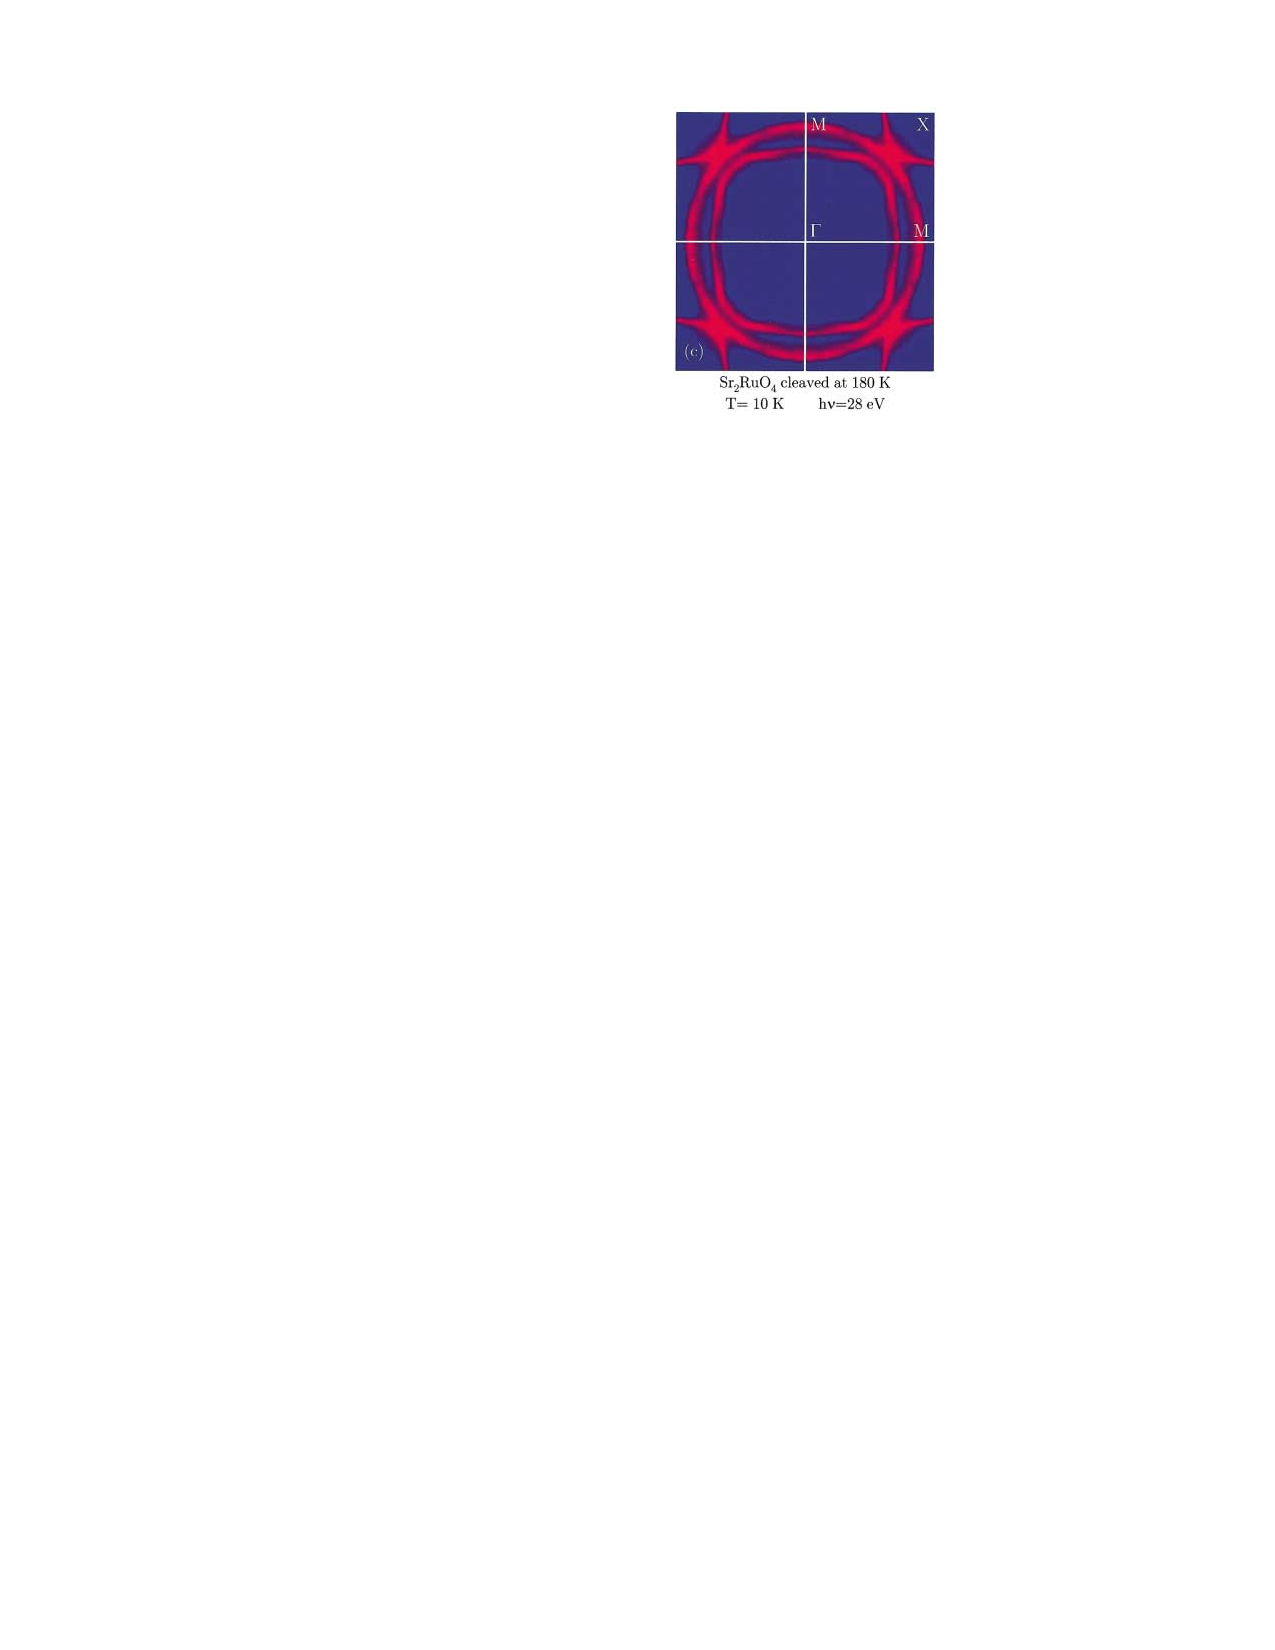
\includegraphics{../resources/SrRuO_FS}

	{\small A. Damascelli et al, PRL \textbf{85} 5194 (2000).}
\end{center}
\end{frame}

\begin{frame}
	\frametitle{强关联电子体系:捉迷藏的费米面}
	\begin{columns}
		\column{.3\textwidth}
		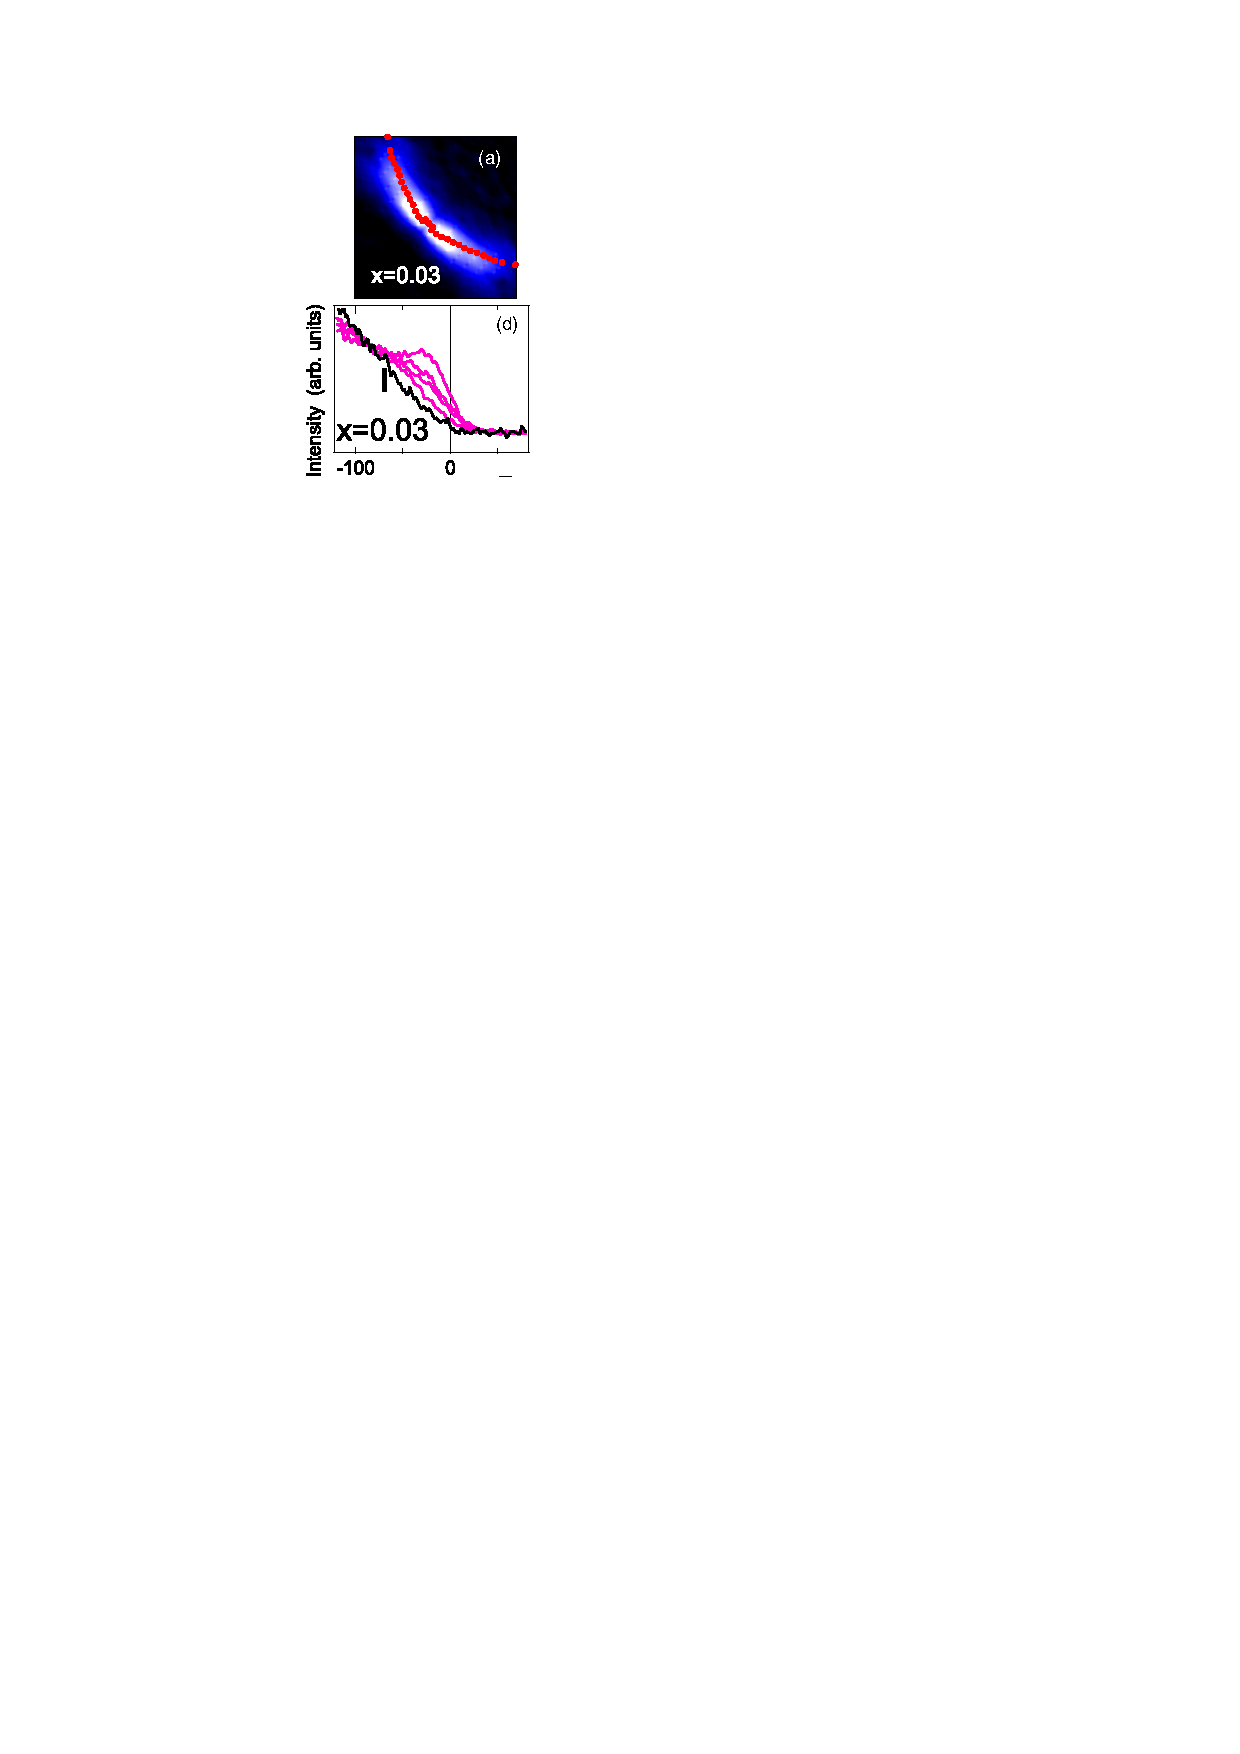
\includegraphics{arc_arpes}
		\column{.7\textwidth}
		\begin{itemize}
			\item 铜基高温超导体: Fermi arc现象。
			\vspace{3em}
			\item 自旋电荷分离: 一种可能的理论解释。
			$c_{i\sigma} = h_i^\dagger f_{i\sigma}$
		\end{itemize}
	\end{columns}
\end{frame}


\begin{frame}
\frametitle{蒙特卡洛模拟得到的相图}
\begin{itemize}
\item 我们设计的模型: $c_{i\alpha} = h_i f_{i\alpha}$, 二者通过格点规范场耦合起来。可以通过大规模行列式量子蒙特卡洛模拟。
\item 费米面藏起来了;
\item 但是通过磁化率响应还能看到。
\end{itemize}
\begin{center}
	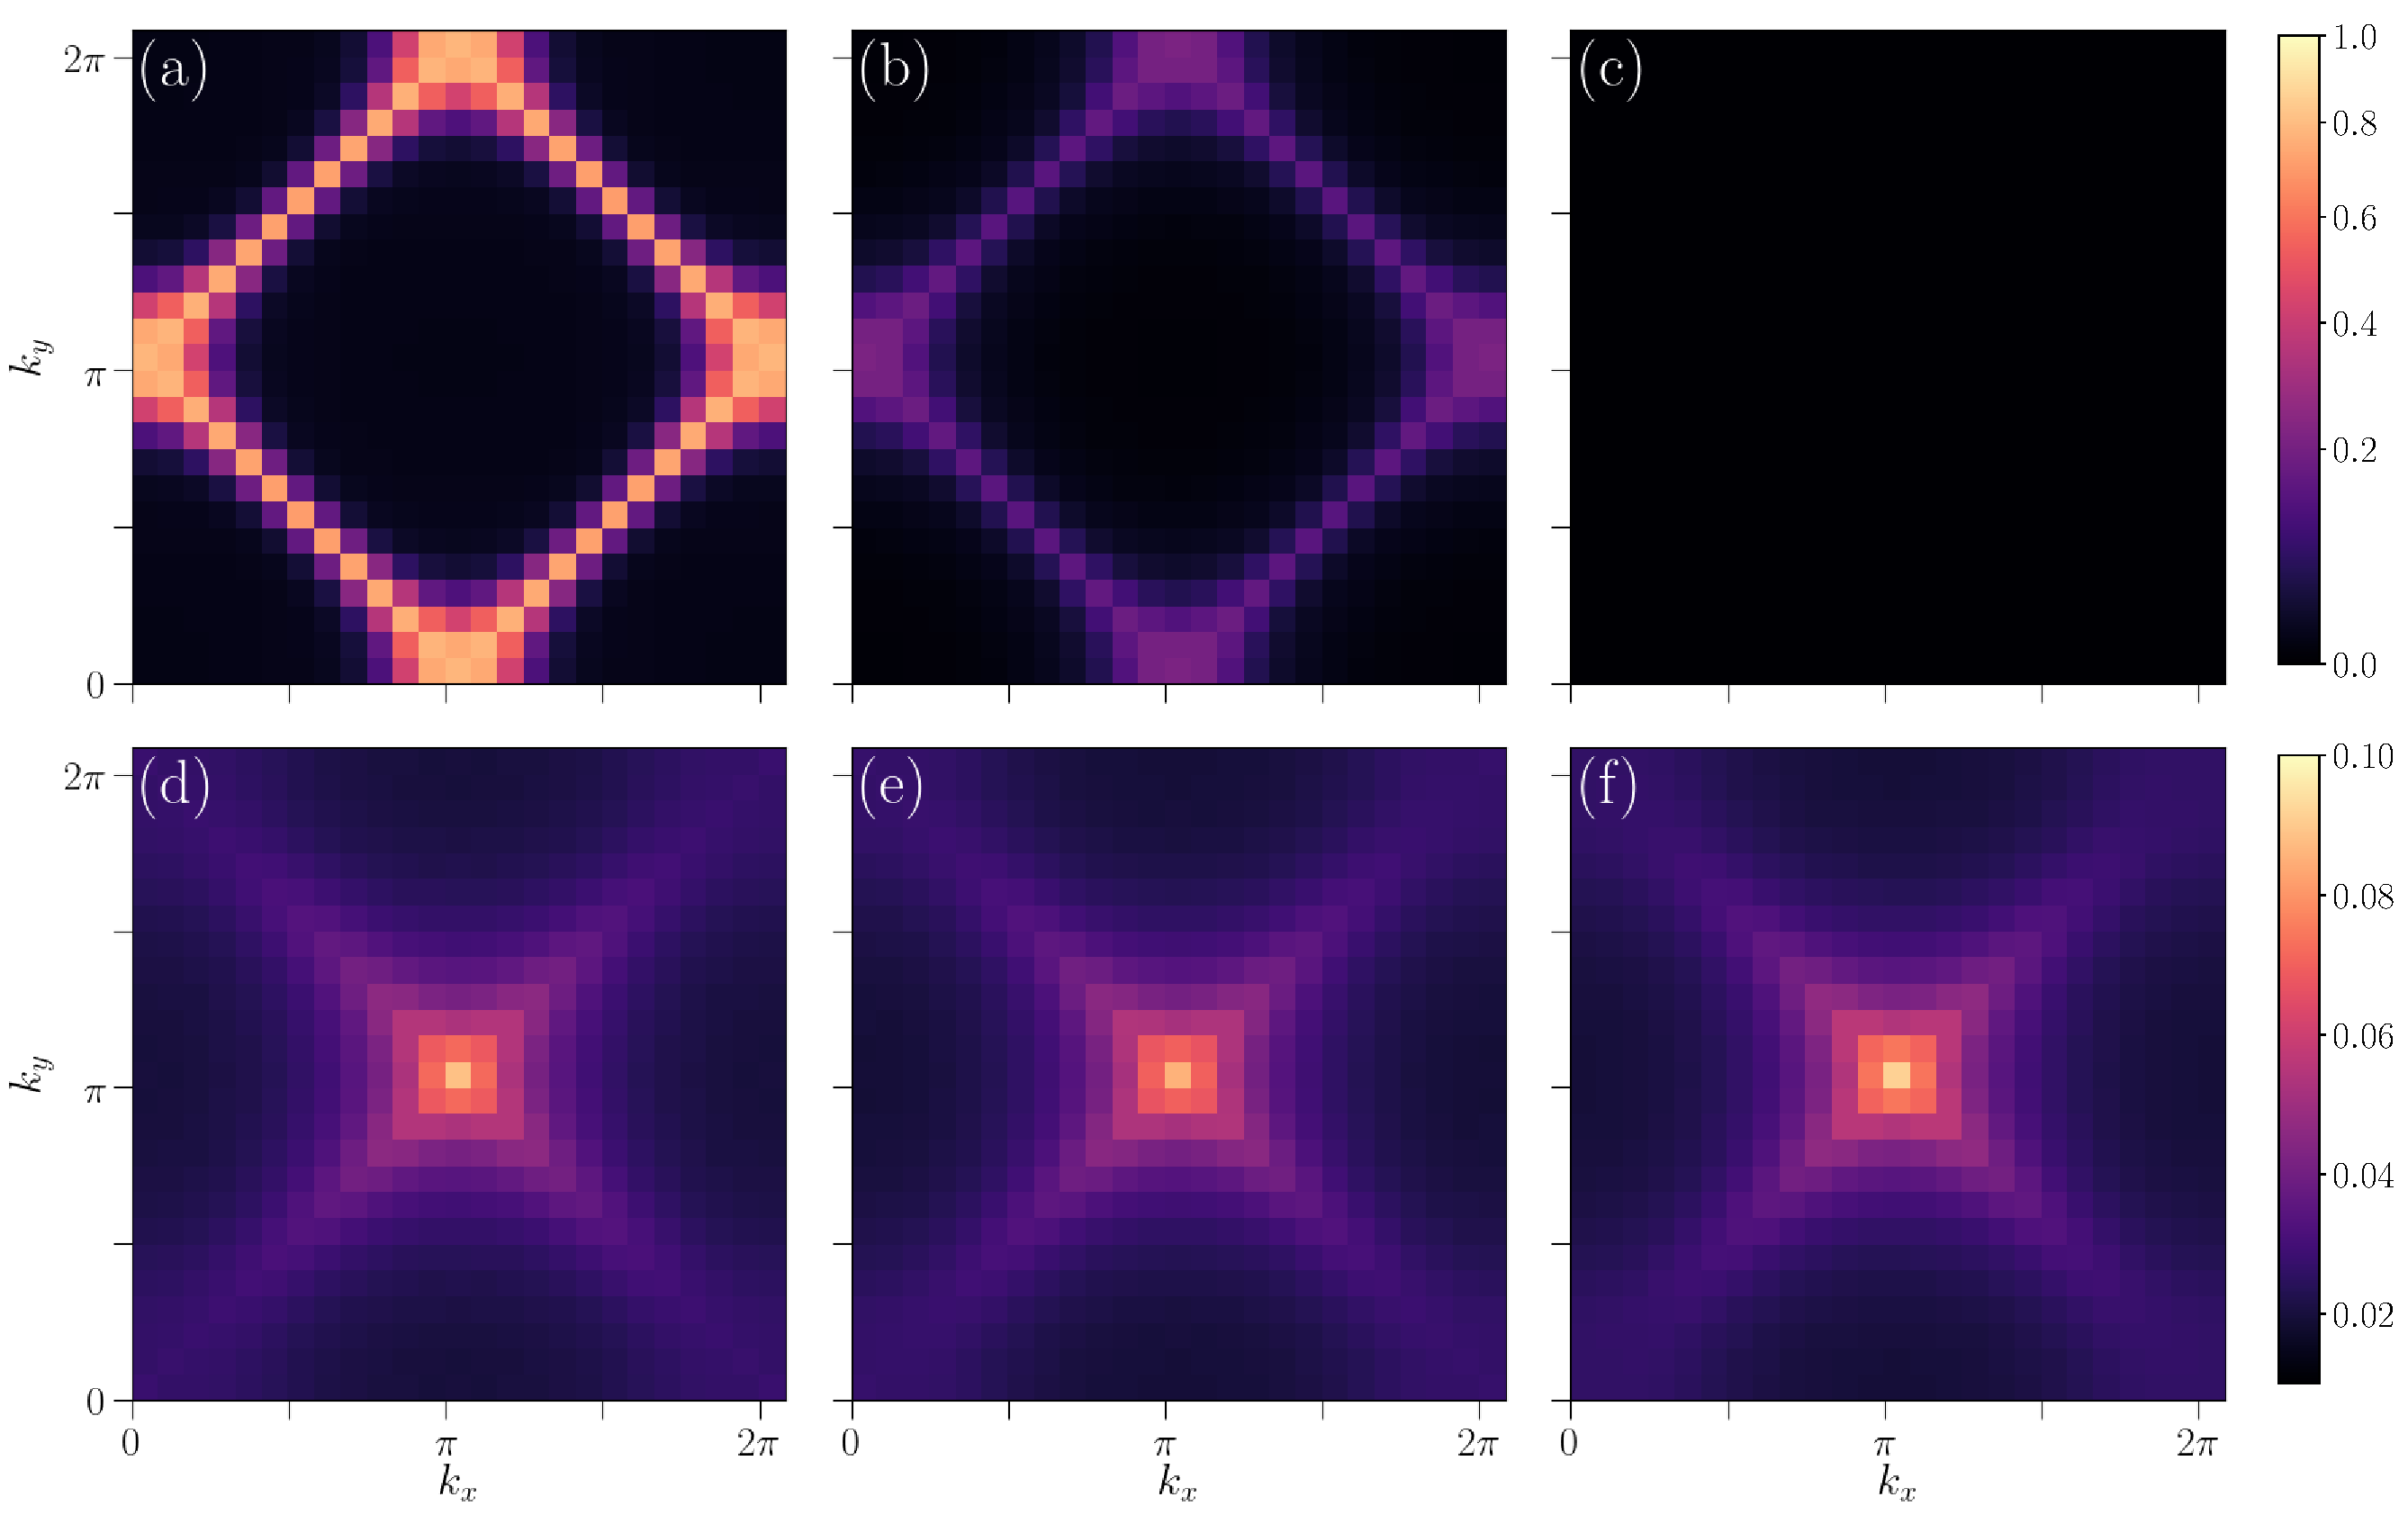
\includegraphics[width=.6\textwidth]{fig2}
\end{center}
\end{frame}

\begin{frame}
	\frametitle{致谢}
	\begin{itemize}
		\item 国家超级计算天津中心:天河一号。
		\item 国家超级计算广州超算中心:天河二号。
		\item 松山湖材料实验室。
		\item 中国物理快报。
	\end{itemize}
	\begin{center}
		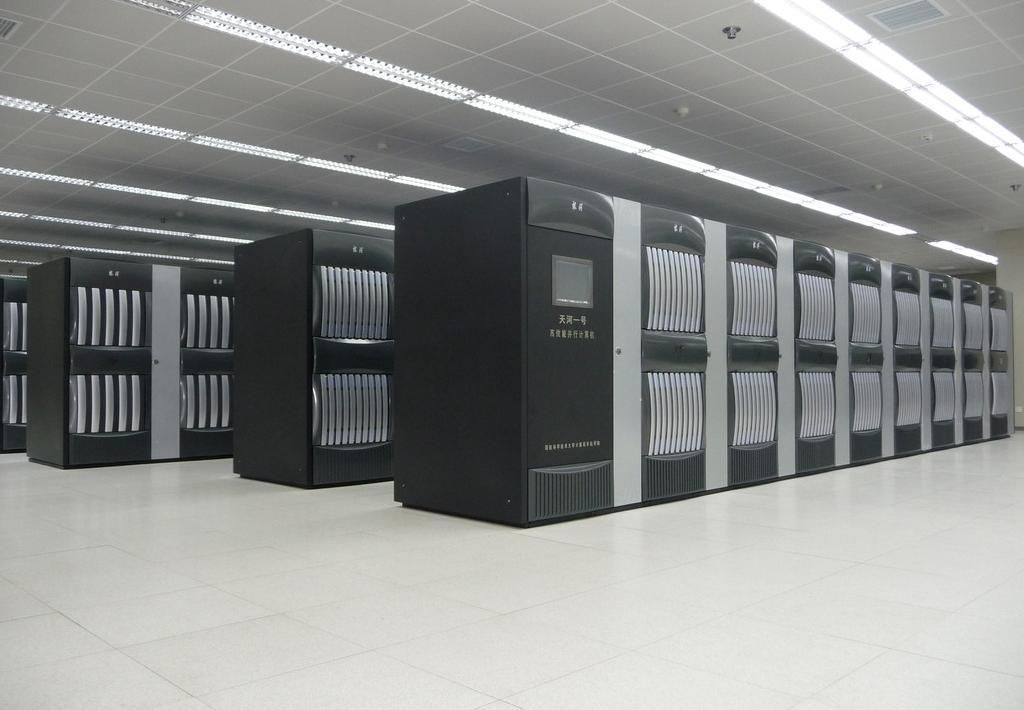
\includegraphics[height=4cm]{../resources/tianhe}
		\hspace{4em}
		\includegraphics[height=4cm]{cpl}
	\end{center}
\end{frame}

\end{document}
